\chapter{Candidate Data Sources}
For the first stage of the pipeline, data ingestion, three data sources will be identified in order to find 
the one that would be most optimal for the production and deployment of a machine learning model to complete 
a supervised learning task. Each data source is thoroughly analysed, answering questions on what the data is, 
why it exists, who it was created by and how it was collected or generated. 

\para Each feature of the candidate datasets is described, including details on what the data in these features 
means. Additionally, the \textbf{type of each feature} is given, describing how the data is quantified in the feature.
Descriptions of types can be found in Table \ref{tab:LevelsOfMeasurement}

\begin{longtable}{ | p{0.1\textwidth} | p{0.5\textwidth} | p{0.3\textwidth} |}
    \hline
    \cellcolor{blue!25}Type & \cellcolor{blue!25}Description & \cellcolor{blue!25}Example data\\
    \hline
    Ratio & Quantitative (numeric) data which measures variables on a continuous scale with a 'true zero' \autocite{careerfoundry_what_2021}.
    & Age\\
    \hline
    Nominal & Data without any inherent relationship or order. Can be qualitative (words, letters) or quantitative \autocite{corporate_finance_institute_nominal_nodate}.
    & Gender, Nationality\\
    \hline 
    Interval & Quantitative data where values are measured at an equal distance (interval) from each other \autocite{dovetail_what_2023}. 
    Differs from ratio data because there is no true zero, with values being able to go below or above it. & Temperature (Celsius), Volume (Decibels)\\
    \hline
    Ordinal & Qualitative data with an inherent relationship, order or sequence \autocite{bhandari_what_2022}. & Survey answers (Strongly disagree, slightly disagree, etc.),
    Levels of education (Bachelor's, Master's, etc.)\\
    \hline
\caption{A brief overview of the different types of data.}\label{tab:LevelsOfMeasurement}
\end{longtable}

\section{Candidate 1 - Indian Liver Patient Dataset}
This dataset \autocite{bendi_ramana_ilpd_2022} consists of real data sourced from hospitals northeast of Andhra Pradesh in India. It was obtained from the
UCI Machine Learning Repository, and has been previously used by \textcite{straw_investigating_2022} in their analysis of sex-related bias in supervised learning models. The UCI ML Repository is a popular host of datasets used by students, 
educators and researchers worldwide for machine learning \autocite{uci_machine_learning_repository_about_nodate}, and hosts these datasets 
on the cloud for public download and usage, as long as credit is given.

\begin{figure}[H]
    \centering
    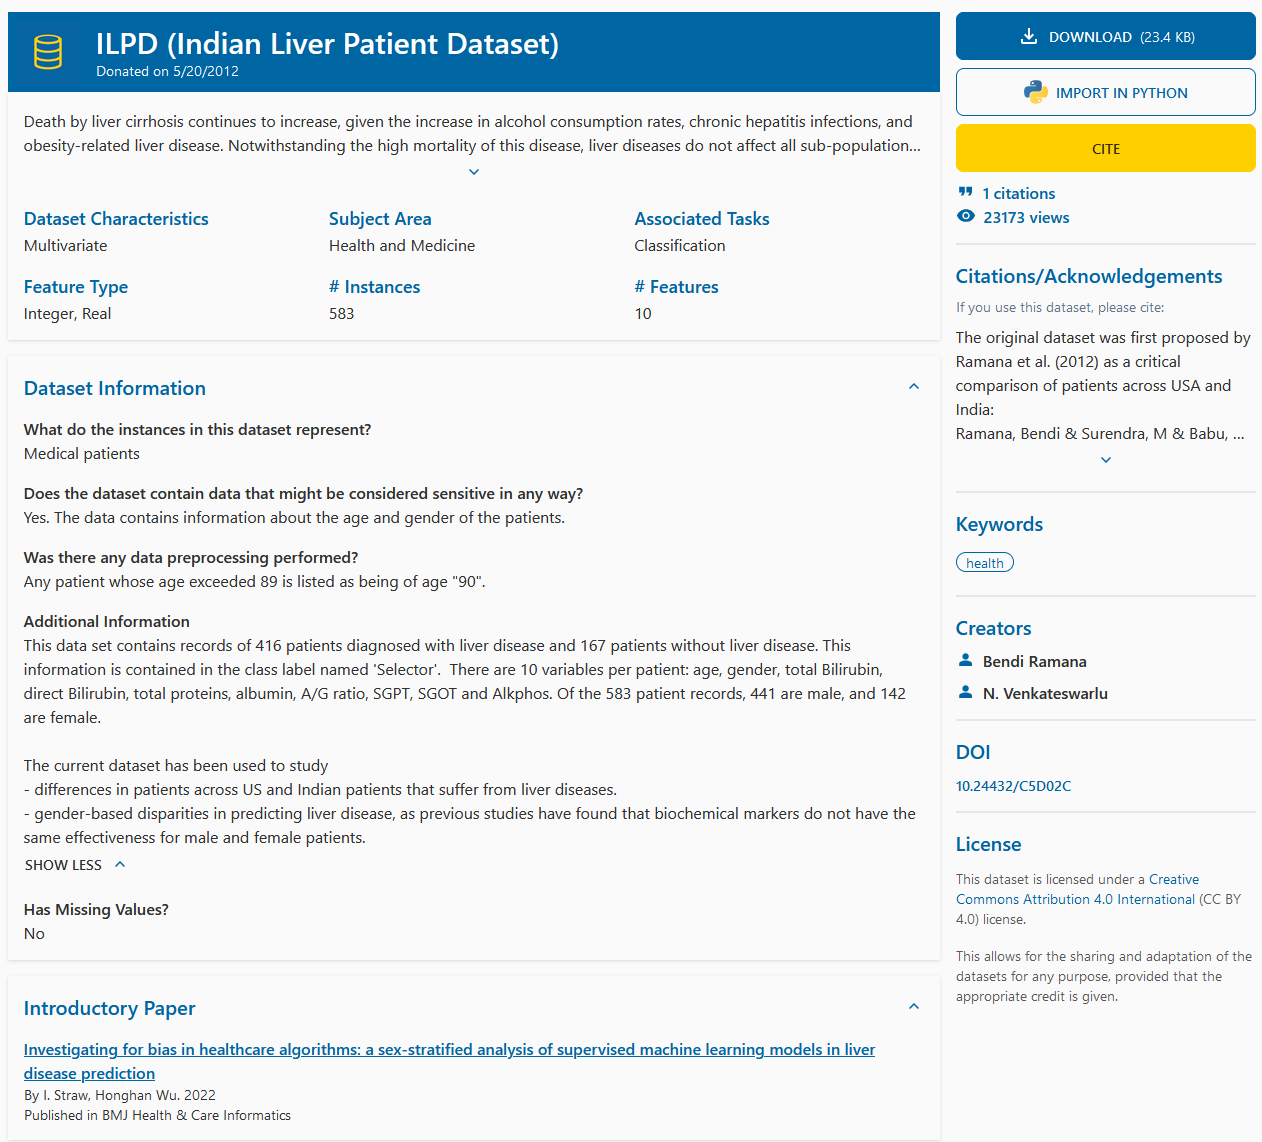
\includegraphics[width=.75\linewidth]{Draft Pipeline/ILPD-UCI.png}
    \caption{A snapshot of the dataset's UCI repository page.}
    \label{fig:ILPD-UCI}
\end{figure}

This dataset in particular aims to assist in the diagnosis of liver
disease due to increasing mortality rates from conditions like liver cirrhosis, and contains 584 records with 10 features
as well as the "Selector" classification column, where those without liver disease are classed as 1, and those with liver disease 
are classed as 2. For the purposes of the ML model, these can be changed to 0 and 1 respectively. 
The dataset is a single flat-file Comma-Separated Values (CSV) file, which stores data by separating each column with commas
and each row with line breaks. This CSV file uses a One Big Table (OBT) schema, as seen in the entity relationship diagram 
in Figure \ref{fig:ILPD-ERD}, wherein all of the data within this dataset is stored in a single table. 
The OBT schema is a denormalised schema that is useful for simple querying due to there being no need for table joins. 
However, it is prone to data duplication and redundancy, which can increase necessary storage requirements.

Descriptions of the columns in the dataset, as well as the associated data types, can be found in Table \ref{tab:ILPD-Types}.

\begin{figure}[H]
    \centering
    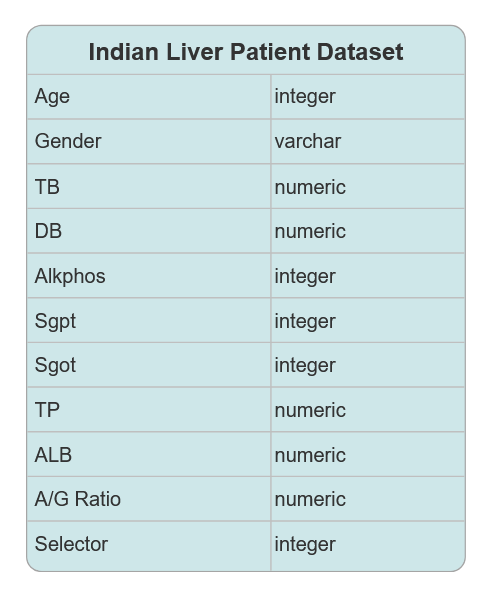
\includegraphics[width=.75\linewidth]{Draft Pipeline/ILPD-ERD.png}
    \caption{An entity relationship diagram of the Indian Liver Patient Dataset.}
    \label{fig:ILPD-ERD}
\end{figure}


A minor issue with this file is that it has no headers in its CSV file, meaning that when imported, Pandas will interpret the first 
row of data as the names of the columns, though this can be combated by adding the "names" argument when calling Pandas' "read\_csv" function,
seen below in Figure \ref{fig:pandasNames}. 

\begin{figure}[H]
    \centering
    \begin{subfigure}{0.75\textwidth}
       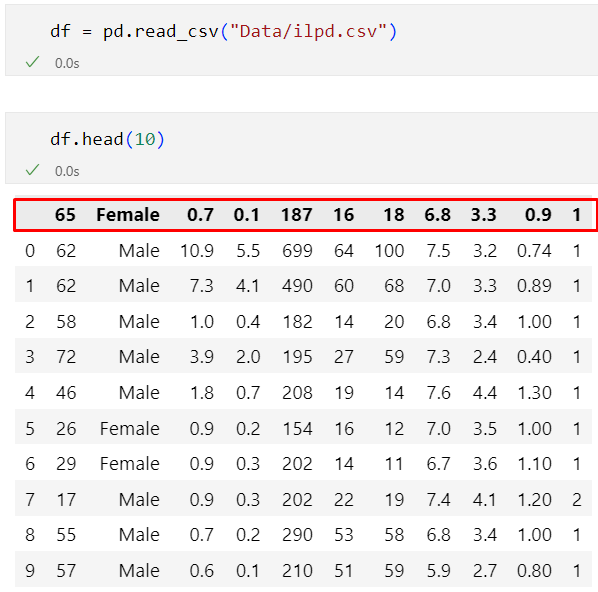
\includegraphics[width=1\linewidth]{Draft Pipeline/pandasNoNames.png}
       \caption{Importing without supplying column names.}
       \label{fig:pandasNames} 
    \end{subfigure}
    
    \begin{subfigure}{1\textwidth}
       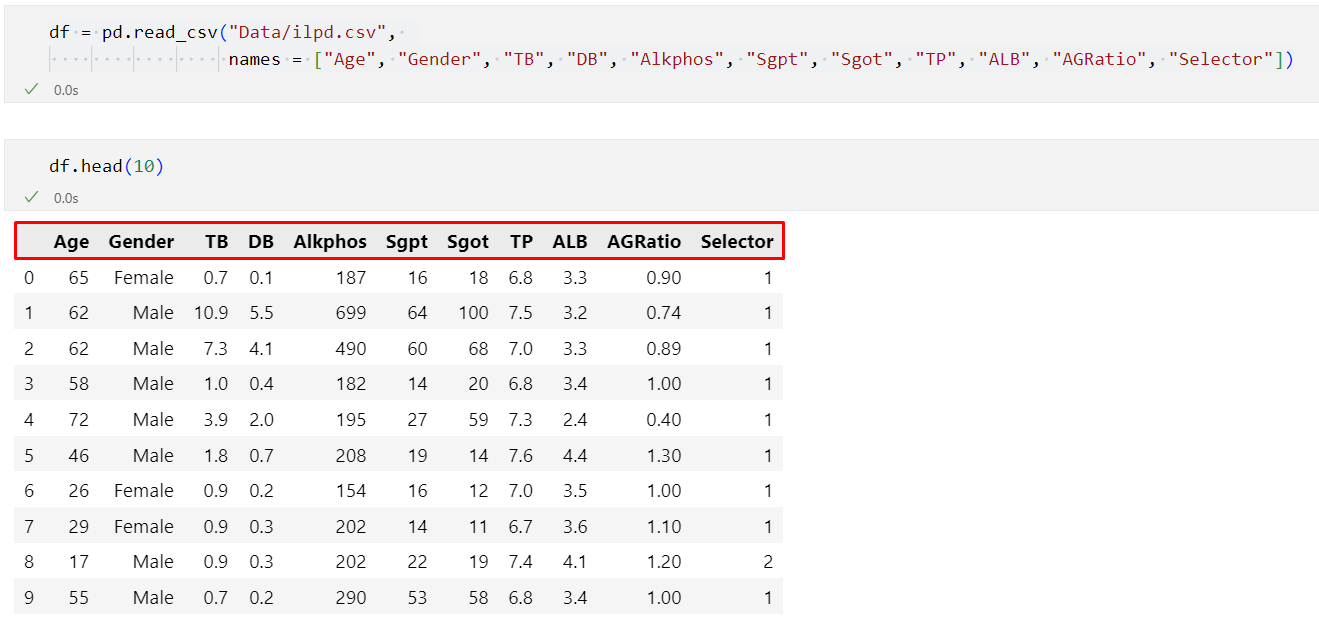
\includegraphics[width=1\linewidth]{Draft Pipeline/pandasNames.png}
       \caption{Importing with the column names.}
       \label{fig:PN2}
    \end{subfigure}
    \caption{Importing and viewing the head of the erroneous CSV using Pandas. The column headers are highlighted in a red box.}
\end{figure}

A preliminary analysis of the file to ascertain the data types of each column, seen in Figure \ref{fig:ILPD-DTypes}, also revealed that there were 4 missing values in the A/G ratio column.
It is possible that these missing values could be imputed rather than deleted, as it may be possible to calculate what the A/G ratio of these rows would have been in the 
Data Preprocessing stage of a pipeline.

\begin{figure}[H]
    \centering
    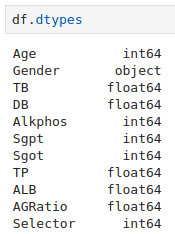
\includegraphics[width=.3\linewidth]{Draft Pipeline/pandas/ILPD-DTypes.png}
    \caption{The data types of the Indian Liver Patient Dataset.}
    \label{fig:ILPD-DTypes}
\end{figure}

\begin{figure}[H]
    \centering
    \begin{subfigure}{0.75\textwidth}
        \centering
       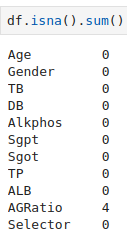
\includegraphics[width=0.3\linewidth]{Draft Pipeline/pandas/ILPD-NA.png}
       \caption{Four missing values are identified.}
       \label{fig:NAs1} 
    \end{subfigure}
    
    \begin{subfigure}{1\textwidth}
        \centering
       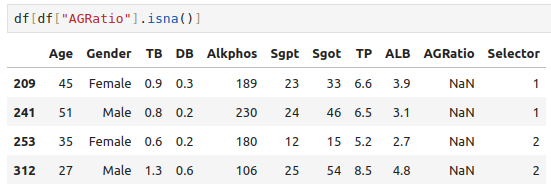
\includegraphics[width=1\linewidth]{Draft Pipeline/pandas/ILPD-NAValues.png}
       \caption{The four rows in question.}
       \label{fig:NAs2}
    \end{subfigure}
    \caption{The identification of four missing values in the A/G ratio column.}
\end{figure}


\begin{table}[H]
    \centering
        \begin{tabular}{ |p{0.2\textwidth}| p{0.4\textwidth}| p{0.2\textwidth}|}
            \hline
            \cellcolor{blue!25}Column & \cellcolor{blue!25}Description & \cellcolor{blue!25}Measurement level\\
            \hline
            Age & The patient's age. \textbf{Ages of 90 or over were listed as 90 before this dataset was published,
            which could introduce a bias in the machine learning model.} 
            & Ratio\\
            \hline
            Gender & The patient's gender, either "Male" or "Female". & Nominal\\
            \hline
            TB & Total bilirubin. Bilirubin is a substance produced by the liver, and a high presence of it may be indicative of
            liver problems \autocite{mayo_clinic_bilirubin_nodate}. & Ratio\\
            \hline
            DB & Direct bilirubin. This is a slightly different form of bilirubin that is formed after the liver has processed it.
            & Ratio\\
            \hline
            Alkphos & Levels of alkaline phosphate - an enzyme in the body produced by the liver. Too much may indicate liver disease. \autocite{clevelandclinic_alkaline_nodate}
            & Ratio\\
            \hline
            Sgpt & Another enzyme found in the liver, where too much can indicate liver problems.
            & Ratio\\
            \hline
            Sgot & Levels of AST in the blood, where too much indicates liver problems.
            & Ratio\\
            \hline
            TP & Total proteins.
            & Ratio\\
            \hline
            ALB & Albumin - a protein in blood plasma. Too little of this may indicate liver problems.
            & Ratio\\
            \hline
            A/G Ratio & The ratio of albumin to globulin, which is another blood protein.
            & Ratio % IS THIS RATIO?
            \\
            \hline
            Selector & The classifier, indicating if the person has liver disease. The target column for the ML model.
            & Nominal\\
            \hline
    \end{tabular}
    \caption{The descriptions of each column in the Indian Liver Patient Dataset.}\label{tab:ILPD-Types}
\end{table}

This dataset could be used to solve a binary classification problem using the ten predictor 
variables and the ground truth Selector column, which will be used in measuring the accuracy of the model. There is a clear 
positive purpose for developing such a model; as previously mentioned, mortality rates from liver disease are high, and an early
diagnosis that could leverage the power of machine learning can greatly enhance the odds of successful treatment.

\pagebreak

\section{Candidate 2 - Spotify Likes Dataset}
This dataset \autocite{vergnou_spotify_nodate} was sourced from \href{https://www.kaggle.com/datasets}{Kaggle}, a platform similar to the UCI ML repository in its 
purpose for students and researchers that acts as a search engine for datasets, but also allows its users to host competitions, upload their machine learning models, and also upload 
their own Python notebooks \autocite{kaggle_kaggle_nodate}. This dataset is stored on their servers on the cloud, and is free to download and use under a 
Creative Commons Public Domain license \autocite{creative_commons_deed_nodate}.

\begin{figure}[H]
    \centering
    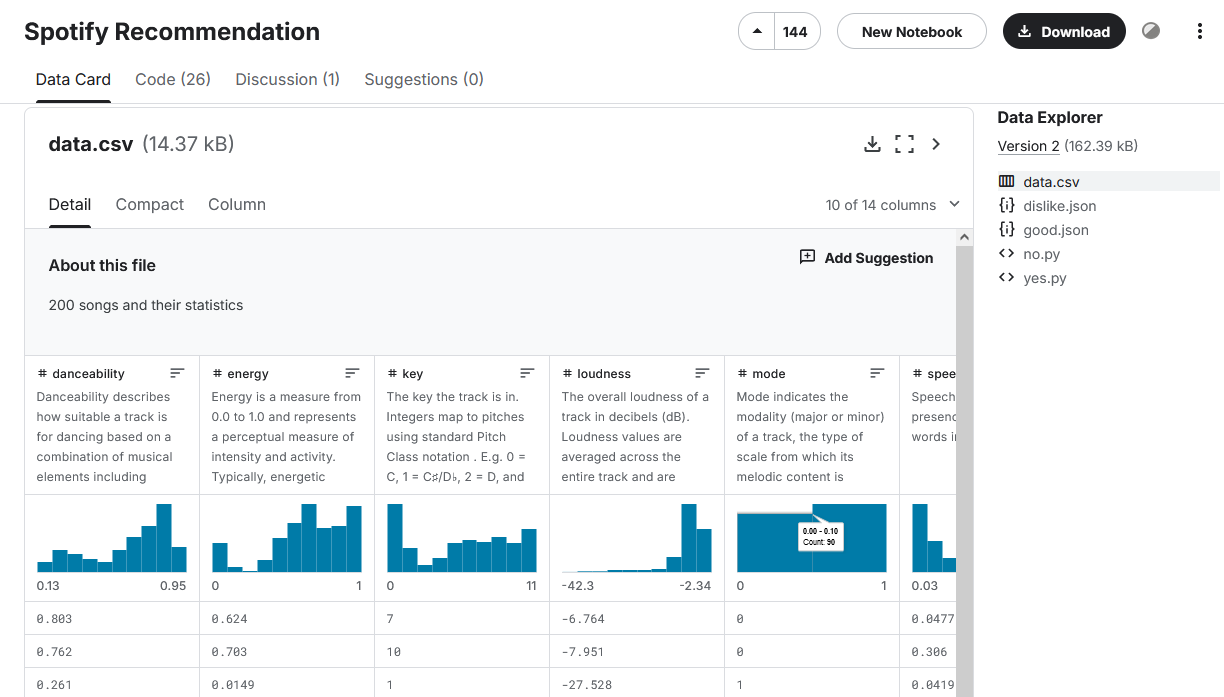
\includegraphics[width=.75\linewidth]{Draft Pipeline/Spotify-Kaggle.png}
    \caption{A snapshot of the Spotify dataset's Kaggle page.}
    \label{fig:Spotify-Kaggle}
\end{figure}

The data itself is split over 
two JavaScript Object Notation (JSON) files, but also fully present in an included CSV file, with all three utilising a One Big Table schema. The 
download also includes two Python files, which have the JSON data stored in Python dictionaries for ease of access, though these will not be used in 
this brief analysis. JSON files store data in \textbf{key-value pairs}, such as in the example snippet of this dataset depicted in Figure \ref{fig:spotifySnippet}.  

\begin{figure}[H]
    \centering
    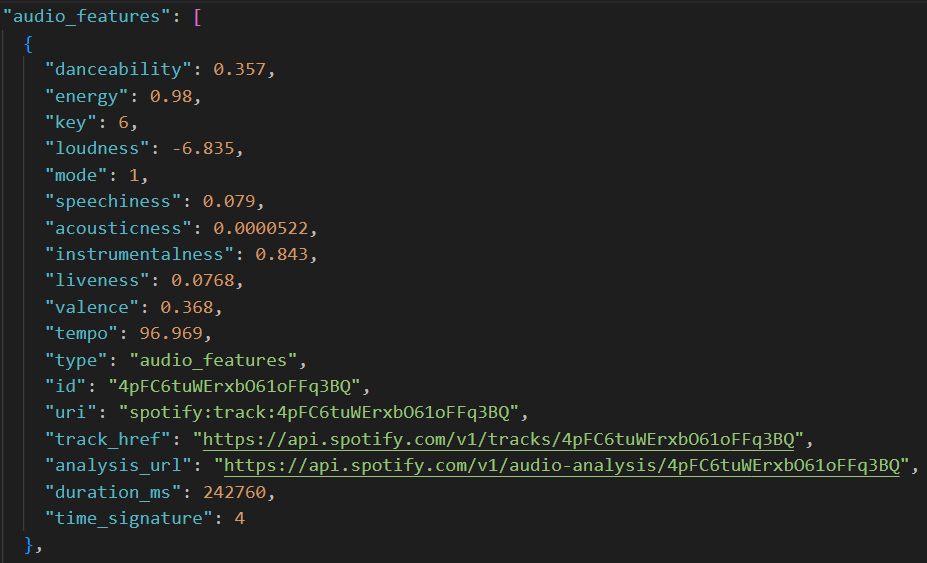
\includegraphics[width=.75\linewidth]{Draft Pipeline/spotifySnippet.png}
    \caption{A snippet of the JSON data, viewed in Visual Studio Code.}
    \label{fig:spotifySnippet}
\end{figure}

Every row in the JSON files is part of the single "audio\_features" key, and each new row is separated by curly braces \{\}. Each column is then given as a 
key-value pair, such as the first row in Figure \ref{fig:spotifySnippet}, where "danceability" is the key, and 0.352 is the associated value.

\noindent This dataset does consist of real data, sourced from the author's personal liked songs directly via the 
\href{https://developer.spotify.com/documentation/web-api}{Spotify API} \autocite{spotify_web_nodate}. There are 195 rows of data, with 100 liked songs, and 95 disliked songs.
Liked and disliked songs are separated into two JSON files, named "dislike" and "good". The two JSON files have 18 features, as depicted in Figure 
\ref{fig:JSON-ERD}. 

\begin{figure}[H]
    \centering
    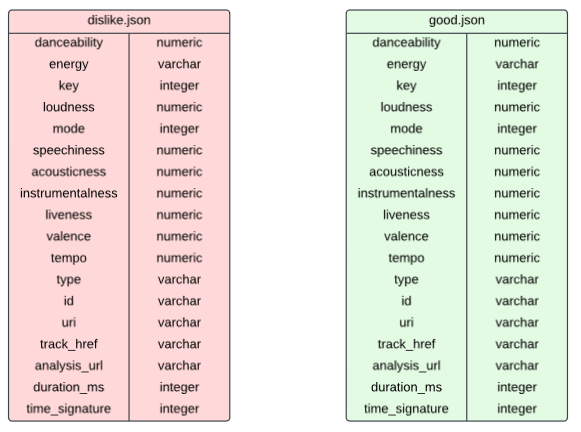
\includegraphics[width=.75\linewidth]{Draft Pipeline/SpotifyJSON-ERD.png}
    \caption{An entity relationship diagram of the two JSON files.}
    \label{fig:JSON-ERD}
\end{figure}

This dataset has been used to create machine learning models before, most notably by its own author, who has a public GitHub repository 
showcasing their work \autocite{brice-vergnou_brice-vergnouspotify_recommendation_2024}. 
Before publicising this data, however, the author had done some preprocessing of their own, having included the additional CSV file,
produced as a result of merging the two JSON files into one CSV and removing unnecessary columns, as depicted in Figure \ref{fig:Spotify-ERD}.
Therefore, my preliminary Pandas analysis of the data types and missing values will only be performed on this CSV, seen in Figures \ref{fig:Spotify-DTypes}
and \ref{fig:Spotify-NA}.

\begin{figure}[H]
    \centering
    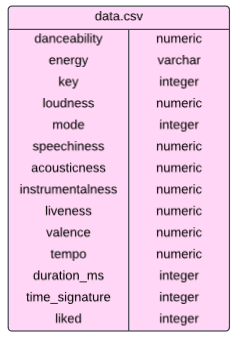
\includegraphics[width=.5\linewidth]{Draft Pipeline/Spotify-ERD.png}
    \caption{An entity relationship diagram of the author's preprocessed CSV file.}
    \label{fig:Spotify-ERD}
\end{figure}

\begin{figure}[H]
    \centering
    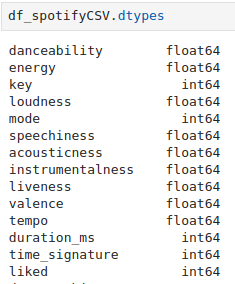
\includegraphics[width=.4\linewidth]{Draft Pipeline/pandas/Spotify-DTypes.png}
    \caption{The data types of the Spotify Likes Dataset.}
    \label{fig:Spotify-DTypes}
\end{figure}

\begin{figure}[H]
    \centering
    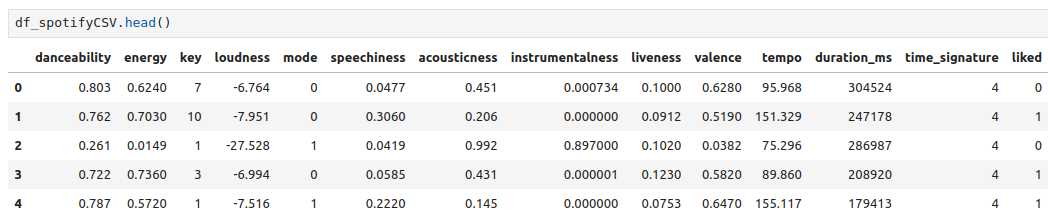
\includegraphics[width=\linewidth]{Draft Pipeline/pandas/Spotify-Head.png}
    \caption{The head of the dataset.}
    \label{fig:Spotify-Head}
\end{figure}

\begin{figure}[H]
    \centering
    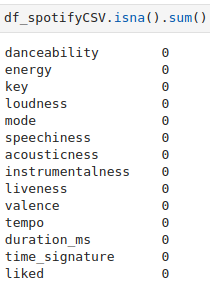
\includegraphics[width=.4\linewidth]{Draft Pipeline/pandas/Spotify-NA.png}
    \caption{No missing values in the dataset.}
    \label{fig:Spotify-NA}
\end{figure}

While a machine learning model to solve a binary classification problem could be trained on this dataset to identify if the author would like a song, 
it has significantly less of a positive impact than Candidates 1 and 3, as this dataset is the author's subjective belief rather than objective
fact that can be applied to other people. Nevertheless, the descriptions of each column can be found in Table \ref{tab:Spotify-Types}.

\begin{table}[H]
    \centering
    \begin{tabular}{ |p{0.2\textwidth}| p{0.45\textwidth}| p{0.2\textwidth}|}
        \hline
        \cellcolor{blue!25}Column & \cellcolor{blue!25}Description & \cellcolor{blue!25}Measurement level\\
            \hline
            Danceability & How suitable a song is for dancing measured from 0.0 to 1.0.
            & Ratio \\
            \hline
            Energy & The intensity and activity of a song. For example, death metal is high energy, whereas classical music is low intensity. 1.0 is the most energetic.
            & Ratio\\
            \hline
            Key & The musical key the song is in, converted to an integer using \href{https://smbutterfield.github.io/ibmt17-18/22-intro-to-non-diatonic-materials/b2-tx-pcintnotation.html}{standard pitch class notation} \autocite{butterfield_22b_nodate}. 
            & Ratio\\
            \hline
            Loudness & The averaged decibel volume of a song, typically between -60 and 0 dB.
            & Interval\\
            \hline
            Mode & Whether a song is in major or minor scale. 1 is major and 0 is minor.
            & Nominal\\
            \hline
            Speechiness & The calculated presence of spoken words in a song.
            & Ratio\\
            \hline
            Acousticness & A confidence measure from 0.0 to 1.0 of whether the track is acoustic. 1.0 represents high confidence the track is acoustic.
            & Ratio\\
            \hline
            Instrumentalness & A confidence measure from 0.0 to 1.0 of whether a song has no vocals.
            & Ratio\\
            \hline
            Liveness & A confidence measure from 0.0 to 1.0 of whether a live audience can be heard as part of a song.
            & Ratio\\
            \hline
            Valence & A confidence measure from 0.0 to 1.0 of the musical positiveness of a song.
            & Ratio\\
            \hline
            Tempo & The beats per minute of a song.
            & Ratio\\
            \hline
            Duration\_MS & The duration of a song in milliseconds.
            & Ratio\\
            \hline
            Time signature & The estimated time signature of the song.
            & Ratio\\
            \hline
            \cellcolor{red!15}Liked & The target variable, indicative of whether the author liked the song or not.
            & Ratio\\
            \hline
            \cellcolor{green!15}Type & Always "audio\_features". Not a relevant predictor.
            & Nominal\\
            \hline
            \cellcolor{green!15}ID & Spotify's own unique ID for a song. Not a relevant predictor.
            & Nominal\\
            \hline
            \cellcolor{green!15}URI & Spotify's URI for the song. Not a relevant predictor.
            & Nominal\\
            \hline
            \cellcolor{green!15}Track HREF & A link to the song on Spotify's API. Not a relevant predictor.
            & Nominal\\  
            \hline
            \cellcolor{green!15}Analysis URL & A link to the song's audio analysis data. Not a relevant predictor. 
            & Nominal\\
            \hline
    \end{tabular}
    \caption{The descriptions of each column in the Spotify songs dataset \autocite{spotify_web_nodate}. Red columns are only present in the CSV, whereas green columns are only present in the JSONs.}\label{tab:Spotify-Types}
\end{table}

These measurements and their descriptions are \href{https://developer.spotify.com/documentation/web-api/reference/get-audio-features}{sourced from Spotify's API},
and are automatically calculated when songs are uploaded to the service. The ground truth of the dataset is present in the CSV file as the "liked" classifier 
column, and a train/test split can be implemented for predictions, which is aided by the fact that this dataset is well balanced (100 liked to 95 disliked).
However, its small size and the fact that the model would only be able to predict one person's specific music taste make 
this dataset a poor candidate. 


\section{Candidate 3 - Loan Approval Classification Dataset}\label{sec:Dataset}
This dataset \autocite{lo_loan_nodate}, similarly to Candidate 2, was sourced from Kaggle's cloud servers under 
an Apache 2.0 license, which states that the dataset can be used as long as credit is given to the original author.
The dataset the physical form of a flat-file CSV, with the logical structure being the One Big Table data 
schema. 

\begin{figure}[H]
    \centering
    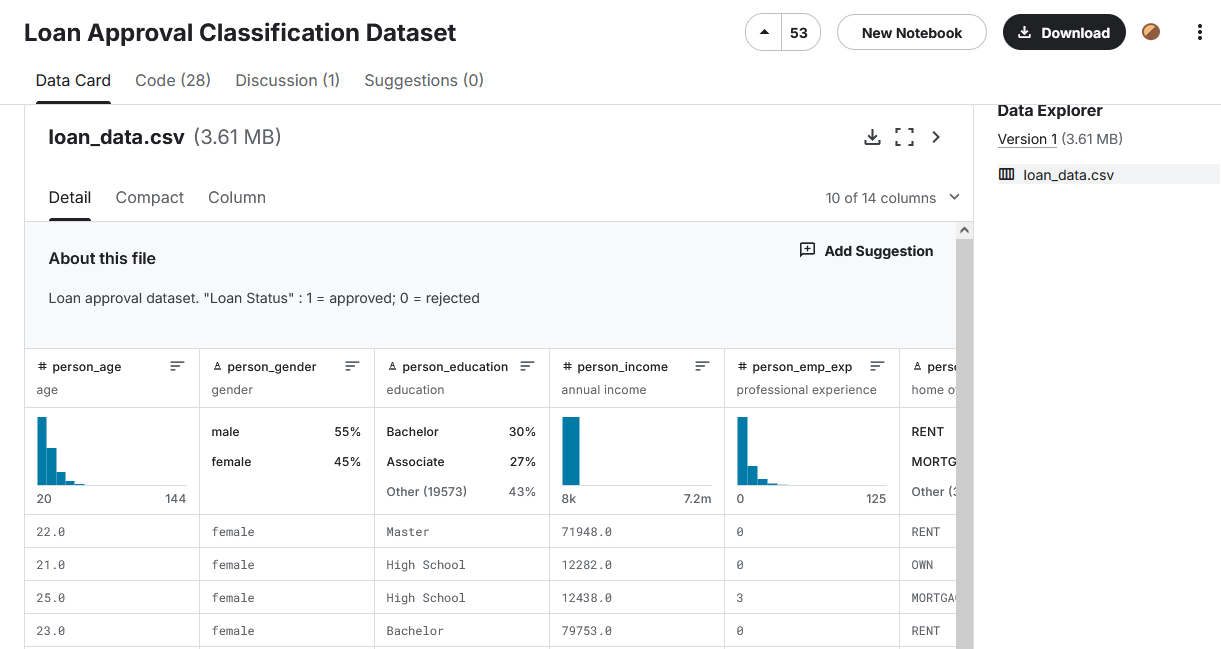
\includegraphics[width=.75\linewidth]{Draft Pipeline/Loan-Kaggle.png}
    \caption{A snapshot of the Loan dataset's Kaggle page.}
    \label{fig:Loan-Kaggle}
\end{figure}

Unlike Candidates 1 and 2, this dataset does not consist of real data, and 
instead consists of synthetic data. This is likely due to the fact that this dataset, if it used real data, would contain extremely personal 
information that could not be shared online due to legislation such as GDPR, which is further discussed in Section \ref{sec:DataHandling}. This particular dataset is an enhanced version of \href{https://www.kaggle.com/datasets/laotse/credit-risk-dataset}{a different credit risk dataset},
which also did not provide an original source and is also presumably synthetic data. The enhancements added were three additional 
columns, for the hypothetical person's gender, education level and credit score. Additionally, the author balanced the dataset using 
Synthetic Minority Oversampling Technique (SMOTE), an oversampling algorithm designed to balance datasets to produce higher
quality machine learning models \autocite{microsoft_smote_2024}.
It can therefore be established that this dataset was created solely for research and analysis purposes, including 
for the creation of supervised learning models. The dataset consists of 45,000 records and 14 features, with 
one of these being the ground truth target variable "loan\_status", which is whether the person should be given a loan or not. 
31 notebooks on Kaggle created by the site's users utilise this dataset, with many of these choosing to solve the binary classification 
problem that it presents, including academic works published by authors such as \textcite{gupta_loanification_2021}. 
The dataset is physically stored as a flat-file CSV, under a One Big Table (OBT) logical data schema.
The data types for each column can be seen in the entity relationship diagram and Pandas code in Figures \ref{fig:Loan-ERD} and \ref{fig:Loan-DTypes}, and 
descriptions of each column can be seen in Table \ref{tab:Loan-Types}.

\begin{figure}[H]
    \centering
    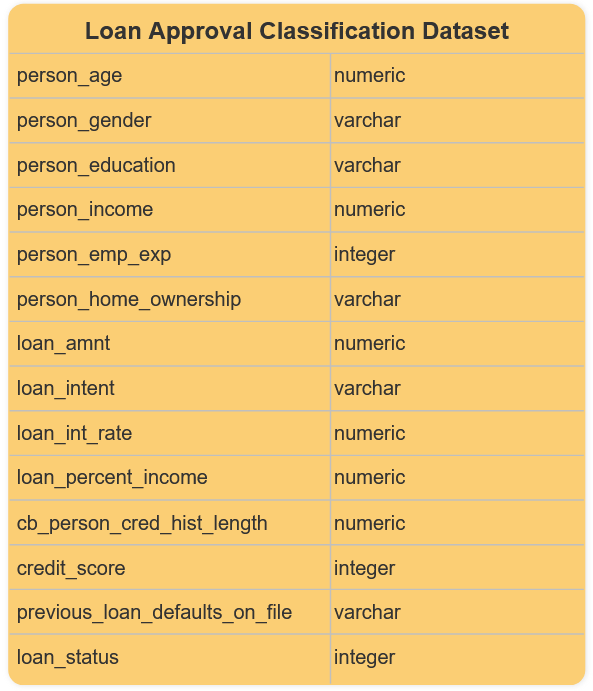
\includegraphics[width=.75\linewidth]{Draft Pipeline/Loan-ERD.png}
    \caption{An entity relationship diagram of the Loan Approval Classification Dataset.}
    \label{fig:Loan-ERD}
\end{figure}

\begin{figure}[H]
    \centering
    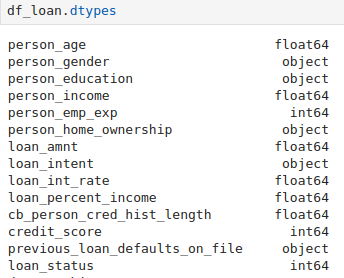
\includegraphics[width=.6\linewidth]{Draft Pipeline/pandas/Loan-DTypes.png}
    \caption{The data types of the Loan Approval Classification Dataset.}
    \label{fig:Loan-DTypes}
\end{figure}

\begin{figure}[H]
    \centering
    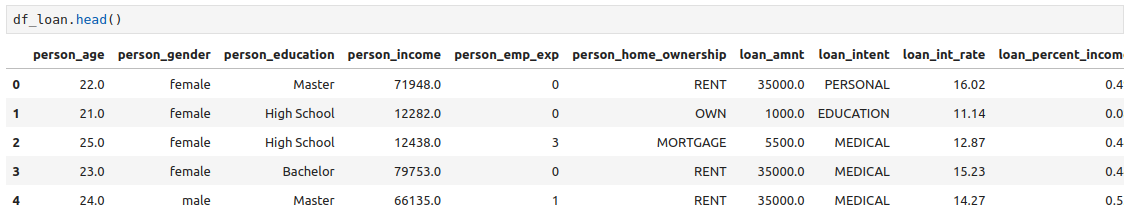
\includegraphics[width=\linewidth]{Draft Pipeline/pandas/Loan-Head.png}
    \caption{The head of the dataset.}
    \label{fig:Loan-Head}
\end{figure}

\begin{figure}[H]
    \centering
    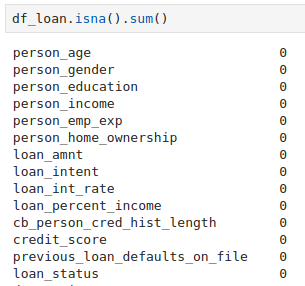
\includegraphics[width=.7\linewidth]{Draft Pipeline/pandas/Loan-NA.png}
    \caption{No missing values in the dataset.}
    \label{fig:Loan-NAs}
\end{figure}


\begin{table}[H]
    \centering
    \begin{tabular}{|p{0.4\textwidth}| p{0.4\textwidth}| p{0.15\textwidth} |}
        \hline
        \cellcolor{blue!25}Column & \cellcolor{blue!25}Description & \cellcolor{blue!25}Measurement level\\
            \hline
            person\_age & The age of the person. & Ratio\\
            \hline
            person\_gender & The person's gender. & Nominal\\
            \hline
            person\_education & The person's highest level of education. & Ordinal\\
            \hline
            person\_emp\_exp & The person's years of employment experience. & Ratio\\
            \hline
            person\_home\_ownership & Home ownership status (for example rent, own, mortgage)
            & Nominal\\
            \hline
            loan\_amnt & The amount of money requested. & Ratio\\
            \hline
            loan\_intent & The purpose of the loan. & Nominal\\
            \hline
            loan\_int\_rate & The interest rate of the loan. & Ratio\\
            \hline
            loan\_percent\_income & Loan amount as a percentage of the person's yearly income.
            & Ratio\\
            \hline
            cb\_person\_cred\_hist\_length & Length of credit history in years. & Ratio\\
            \hline
            credit\_score & Credit score of the person. & Ratio\\
            \hline
            previous\_loan\_defaults\_on\_file & If the person has defaulted on a loan before.
            & Nominal \\
            \hline
            loan\_status & Whether the loan should be approved. 1 if yes, 0 if no.
            & Nominal\\
            \hline
    \end{tabular}
    \caption{The descriptions of each column in the dataset.}\label{tab:Loan-Types}
\end{table}

This dataset is also frequently updated, with its most recent update occurring on the 29th of October.
This would mean it may be more suited to an OLTP database system, which will be further discussed in Section 
\ref{sec:Ingestion}.

\section{Chosen dataset}
Of the three candidates presented, the most suitable for a machine learning operations pipeline would be Candidate 3, the loan approval dataset. As mentioned 
in Section \ref{sec:Dataset}, this dataset possesses many predictor variables and an adequate amount of data to train a supervised learning classification model 
to classify whether an individual should be allowed a loan or not. While the data in this dataset is synthetic due to its real equivalent being highly protected 
under data protection legislation, the model trained from said synthetic data could be applied to real data using what it has learned, and could greatly expedite 
the process of loan approvals.

As previously mentioned, the dataset is hosted on Kaggle's cloud database, in the physical structure of a  
CSV file, using a One Big Table (OBT) data schema for its logical structure.  
Libraries such as Pandas natively work with these types of files which will allow for quick ingestion. 
When the dataset is ingested, it will be stored in a MariaDB Columnstore instance, which is further 
described in Section \ref{ch:PlanMLOps}. For this pipeline, the data will be kept in the OBT schema
due to the simplicity and efficiency of queries performed on it, and also to ensure maximum data integrity
that could be lost if the logical structure were modified. There were other options that could have been used
instead of OBT, represented in Table \ref{tab:Schemas}.


\begin{longtable}{ |p{0.15\textwidth}| p{0.22\textwidth}| p{0.2\textwidth} | p{0.25\textwidth} | }
    \hline
    \cellcolor{blue!25}Schema & \cellcolor{blue!25}Description & \cellcolor{blue!25}Positives & \cellcolor{blue!25}Negatives \\
    \hline
    Star
    \autocite{kaminsky_star_nodate} & Stores data across a main fact table for measured or transactional data, and dimension tables 
    for data related to the fact data, which can be visualised like a star. & Simple to understand, few joins needed,
    very scalable. & Data updates would require updates of multiple rows in multiple tables. Adding new columns
    (dimensions) after initial creation can be difficult because the schema is denormalised.\\
    \hline
    Snowflake
    \autocite{geeksforgeeks_snowflake_2023} & An extended form of the Star schema that further branches its dimension tables
    into a hierarchy, appearing more like a snowflake than a star due to the multiple branches formed. &
    Unlike a star schema, data is normalised, allowing data to be added easier than a star schema. & More 
    complex to query due to the increased amount of tables, therefore requiring more processing power. \\
    \hline
    Normalised Relational Model 
    \autocite{microsoft_database_2024} & Heavily organises data, and emphasises the relationships between tables. &
    Keeps minimal or no redundant data whatsoever, reducing storage requirements. In doing so, this also heightens 
    data integrity. & As with other schemas that use many tables, queries can be slowed by the need for multiple 
    joins. \\
    \hline 
    \caption{An analysis of alternative data schemas.}\label{tab:Schemas}
\end{longtable}


\chapter{Planning the MLOps Pipeline}\label{ch:PlanMLOps}
All machine learning operations (MLOps) follow a five-step repeatable pipeline, outlined in Figure \ref{fig:MLPipeline}, where the output of one stage
becomes the input of the next. 
\begin{figure}[H]
    \centering
    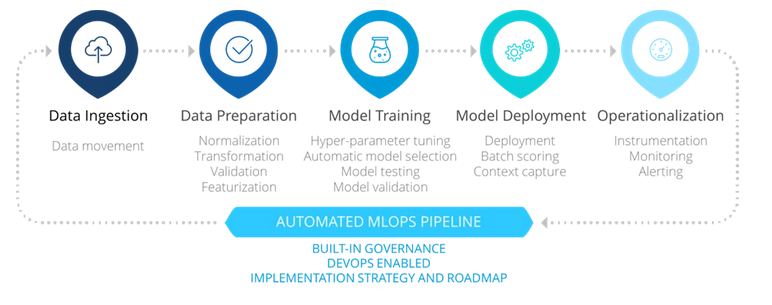
\includegraphics[width=.75\linewidth]{Draft Pipeline/MLPipeline.png}
    \caption{The five key steps in an MLOps pipeline \autocite{incycle_software_mlops_nodate}.}
    \label{fig:MLPipeline}
\end{figure}
The pipeline begins with raw data and finishes with a trained machine learning model, and is often 
repeated at certain intervals, which could be as simple as once a day, or it could be repeated as new data becomes available. 
This repetition is performed automatically, so that the final model can become progressively more accurate. Because the process 
must be repeatable and automated, it is essential that data is validated to ensure that one run of the pipeline where the data may have 
been corrupted somehow would not cause issues, which would quickly spiral out of control as the pipeline is repeated again and again.
Overall, MLOps pipelines standardise the development and deployment process of machine learning models, ensuring continuous integration
(CI) and continuous delivery (CD) and enhancing collaboration between data scientists and development teams.

\pagebreak